% Options for packages loaded elsewhere
\PassOptionsToPackage{unicode}{hyperref}
\PassOptionsToPackage{hyphens}{url}
%
\documentclass[
]{article}
\usepackage{amsmath,amssymb}
\usepackage{lmodern}
\usepackage{ifxetex,ifluatex}
\ifnum 0\ifxetex 1\fi\ifluatex 1\fi=0 % if pdftex
  \usepackage[T1]{fontenc}
  \usepackage[utf8]{inputenc}
  \usepackage{textcomp} % provide euro and other symbols
\else % if luatex or xetex
  \usepackage{unicode-math}
  \defaultfontfeatures{Scale=MatchLowercase}
  \defaultfontfeatures[\rmfamily]{Ligatures=TeX,Scale=1}
\fi
% Use upquote if available, for straight quotes in verbatim environments
\IfFileExists{upquote.sty}{\usepackage{upquote}}{}
\IfFileExists{microtype.sty}{% use microtype if available
  \usepackage[]{microtype}
  \UseMicrotypeSet[protrusion]{basicmath} % disable protrusion for tt fonts
}{}
\makeatletter
\@ifundefined{KOMAClassName}{% if non-KOMA class
  \IfFileExists{parskip.sty}{%
    \usepackage{parskip}
  }{% else
    \setlength{\parindent}{0pt}
    \setlength{\parskip}{6pt plus 2pt minus 1pt}}
}{% if KOMA class
  \KOMAoptions{parskip=half}}
\makeatother
\usepackage{xcolor}
\IfFileExists{xurl.sty}{\usepackage{xurl}}{} % add URL line breaks if available
\IfFileExists{bookmark.sty}{\usepackage{bookmark}}{\usepackage{hyperref}}
\hypersetup{
  pdftitle={Laboratorio statistico informatico},
  pdfauthor={null},
  hidelinks,
  pdfcreator={LaTeX via pandoc}}
\urlstyle{same} % disable monospaced font for URLs
\usepackage[margin=1in]{geometry}
\usepackage{color}
\usepackage{fancyvrb}
\newcommand{\VerbBar}{|}
\newcommand{\VERB}{\Verb[commandchars=\\\{\}]}
\DefineVerbatimEnvironment{Highlighting}{Verbatim}{commandchars=\\\{\}}
% Add ',fontsize=\small' for more characters per line
\usepackage{framed}
\definecolor{shadecolor}{RGB}{248,248,248}
\newenvironment{Shaded}{\begin{snugshade}}{\end{snugshade}}
\newcommand{\AlertTok}[1]{\textcolor[rgb]{0.94,0.16,0.16}{#1}}
\newcommand{\AnnotationTok}[1]{\textcolor[rgb]{0.56,0.35,0.01}{\textbf{\textit{#1}}}}
\newcommand{\AttributeTok}[1]{\textcolor[rgb]{0.77,0.63,0.00}{#1}}
\newcommand{\BaseNTok}[1]{\textcolor[rgb]{0.00,0.00,0.81}{#1}}
\newcommand{\BuiltInTok}[1]{#1}
\newcommand{\CharTok}[1]{\textcolor[rgb]{0.31,0.60,0.02}{#1}}
\newcommand{\CommentTok}[1]{\textcolor[rgb]{0.56,0.35,0.01}{\textit{#1}}}
\newcommand{\CommentVarTok}[1]{\textcolor[rgb]{0.56,0.35,0.01}{\textbf{\textit{#1}}}}
\newcommand{\ConstantTok}[1]{\textcolor[rgb]{0.00,0.00,0.00}{#1}}
\newcommand{\ControlFlowTok}[1]{\textcolor[rgb]{0.13,0.29,0.53}{\textbf{#1}}}
\newcommand{\DataTypeTok}[1]{\textcolor[rgb]{0.13,0.29,0.53}{#1}}
\newcommand{\DecValTok}[1]{\textcolor[rgb]{0.00,0.00,0.81}{#1}}
\newcommand{\DocumentationTok}[1]{\textcolor[rgb]{0.56,0.35,0.01}{\textbf{\textit{#1}}}}
\newcommand{\ErrorTok}[1]{\textcolor[rgb]{0.64,0.00,0.00}{\textbf{#1}}}
\newcommand{\ExtensionTok}[1]{#1}
\newcommand{\FloatTok}[1]{\textcolor[rgb]{0.00,0.00,0.81}{#1}}
\newcommand{\FunctionTok}[1]{\textcolor[rgb]{0.00,0.00,0.00}{#1}}
\newcommand{\ImportTok}[1]{#1}
\newcommand{\InformationTok}[1]{\textcolor[rgb]{0.56,0.35,0.01}{\textbf{\textit{#1}}}}
\newcommand{\KeywordTok}[1]{\textcolor[rgb]{0.13,0.29,0.53}{\textbf{#1}}}
\newcommand{\NormalTok}[1]{#1}
\newcommand{\OperatorTok}[1]{\textcolor[rgb]{0.81,0.36,0.00}{\textbf{#1}}}
\newcommand{\OtherTok}[1]{\textcolor[rgb]{0.56,0.35,0.01}{#1}}
\newcommand{\PreprocessorTok}[1]{\textcolor[rgb]{0.56,0.35,0.01}{\textit{#1}}}
\newcommand{\RegionMarkerTok}[1]{#1}
\newcommand{\SpecialCharTok}[1]{\textcolor[rgb]{0.00,0.00,0.00}{#1}}
\newcommand{\SpecialStringTok}[1]{\textcolor[rgb]{0.31,0.60,0.02}{#1}}
\newcommand{\StringTok}[1]{\textcolor[rgb]{0.31,0.60,0.02}{#1}}
\newcommand{\VariableTok}[1]{\textcolor[rgb]{0.00,0.00,0.00}{#1}}
\newcommand{\VerbatimStringTok}[1]{\textcolor[rgb]{0.31,0.60,0.02}{#1}}
\newcommand{\WarningTok}[1]{\textcolor[rgb]{0.56,0.35,0.01}{\textbf{\textit{#1}}}}
\usepackage{graphicx}
\makeatletter
\def\maxwidth{\ifdim\Gin@nat@width>\linewidth\linewidth\else\Gin@nat@width\fi}
\def\maxheight{\ifdim\Gin@nat@height>\textheight\textheight\else\Gin@nat@height\fi}
\makeatother
% Scale images if necessary, so that they will not overflow the page
% margins by default, and it is still possible to overwrite the defaults
% using explicit options in \includegraphics[width, height, ...]{}
\setkeys{Gin}{width=\maxwidth,height=\maxheight,keepaspectratio}
% Set default figure placement to htbp
\makeatletter
\def\fps@figure{htbp}
\makeatother
\setlength{\emergencystretch}{3em} % prevent overfull lines
\providecommand{\tightlist}{%
  \setlength{\itemsep}{0pt}\setlength{\parskip}{0pt}}
\setcounter{secnumdepth}{-\maxdimen} % remove section numbering
\ifluatex
  \usepackage{selnolig}  % disable illegal ligatures
\fi

\title{Laboratorio statistico informatico}
\author{null}
\date{29/8/2021}

\begin{document}
\maketitle

\hypertarget{introduzione}{%
\subsubsection{Introduzione}\label{introduzione}}

Nel seguente report vengono approfonditi, come da richiesta, alcuni
degli aspetti relativi al progetto 1. In seguito si riporta la consegna:

\begin{quote}
Il report (di lunghezza 2000-3000 parole, esclusi grafici e tabelle)
dovrà contenere:

\begin{itemize}
\item
  Una spiegazione delle formule utilizzate per calcolare il premio e per
  l'evoluzione del fondo;
\item
  Il codice e una spiegazione della logica utilizzata nella sua
  preparazione;
\item
  Alcuni esempi che illustrino la versatilità della funzione in 1);
\item
  Con riferimento a un dato esempio (es. rendita differita immediata
  temporanea), utilizzare il metodo Monte Carlo per valutare la
  distribuzione del fondo all'ultima epoca disponibile (valore atteso,
  deviazione standard, altri momenti, quantili, probabilità di rovina
  (fondo negativo), etc.).
\end{itemize}
\end{quote}

\hypertarget{la-funzione}{%
\subsubsection{La funzione}\label{la-funzione}}

\begin{Shaded}
\begin{Highlighting}[]
\FunctionTok{library}\NormalTok{(lifecontingencies)}
\end{Highlighting}
\end{Shaded}

\begin{verbatim}
## Package:  lifecontingencies
## Authors:  Giorgio Alfredo Spedicato [aut, cre]
##     (<https://orcid.org/0000-0002-0315-8888>),
##   Christophe Dutang [ctb] (<https://orcid.org/0000-0001-6732-1501>),
##   Reinhold Kainhofer [ctb] (<https://orcid.org/0000-0002-7895-1311>),
##   Kevin J Owens [ctb],
##   Ernesto Schirmacher [ctb],
##   Gian Paolo Clemente [ctb] (<https://orcid.org/0000-0001-6795-4595>),
##   Ivan Williams [ctb]
## Version:  1.3.7
## Date:     2021-03-21 22:00:02 UTC
## BugReport: https://github.com/spedygiorgio/lifecontingencies/issues
\end{verbatim}

\begin{Shaded}
\begin{Highlighting}[]
\CommentTok{\#\textquotesingle{} Gestione Portafoglio}
\CommentTok{\#\textquotesingle{} Dato un portafoglio, di rischi omogenei tra loro, la funzione calcola rendimento e andamento del fondo e i decessi }
\CommentTok{\#\textquotesingle{}}
\CommentTok{\#\textquotesingle{} @param numeroAssicurati }
\CommentTok{\#\textquotesingle{} @param eta età degli assicurati}
\CommentTok{\#\textquotesingle{} @param rata importo della rata annuale}
\CommentTok{\#\textquotesingle{} @param fondoInizio importo iniziale del fondo}
\CommentTok{\#\textquotesingle{} @param numeroPremi numero di premi che gli assicurati pagheranno}
\CommentTok{\#\textquotesingle{} @param omega età massima raggiungibile}
\CommentTok{\#\textquotesingle{} @param differimento rendita differita o immediata}
\CommentTok{\#\textquotesingle{} @param temporanea rendita vitalizia o temporanea}
\CommentTok{\#\textquotesingle{} @param anniCopertura anni di coperrtura nel caso di rendita temporanea}
\CommentTok{\#\textquotesingle{} @param rateGarantiteDurata numero di rate garantite}
\CommentTok{\#\textquotesingle{} @param rendimentoFondoAnnuo tasso di rendimento del fondo }
\CommentTok{\#\textquotesingle{} @param tassoAleatorio tasso fisso o aleatorio}
\CommentTok{\#\textquotesingle{} @param tavolaMortalita tavola di mortalità con cui calcolare il premio}
\CommentTok{\#\textquotesingle{} @param tassoTecnico tasso usato per calcolare il premio}
\CommentTok{\#\textquotesingle{} @param tavolaPeriodo tavola utilizzata per simulare i decessi all\textquotesingle{}interno del portafoglio}
\CommentTok{\#\textquotesingle{}}
\CommentTok{\#\textquotesingle{} @return}
\CommentTok{\#\textquotesingle{} La funzione ritorna l\textquotesingle{}andamento e il rendimento del fondo, i decessi e il premio che ciascun assicurato dovrà pagare}
\CommentTok{\#\textquotesingle{} }
\CommentTok{\#\textquotesingle{} @export}
\CommentTok{\#\textquotesingle{}}
\CommentTok{\#\textquotesingle{} @examples}
\NormalTok{gestionePortafoglio }\OtherTok{=} \ControlFlowTok{function}\NormalTok{(}\CommentTok{\#input}
  \AttributeTok{numeroAssicurati =} \DecValTok{1000}\NormalTok{,}
  \AttributeTok{eta =} \DecValTok{20}\NormalTok{,}
  \AttributeTok{rata =} \DecValTok{1000}\NormalTok{,}
  \AttributeTok{fondoInizio =} \DecValTok{100000}\NormalTok{,}
  \AttributeTok{numeroPremi =} \DecValTok{15}\NormalTok{,}
  \AttributeTok{omega =} \DecValTok{110}\NormalTok{,}
  \AttributeTok{differimento =} \DecValTok{25}\NormalTok{,}
  \AttributeTok{temporanea =} \ConstantTok{FALSE}\NormalTok{,}
  \CommentTok{\# temporanea o  vita intera}
  \AttributeTok{anniCopertura =} \DecValTok{35}\NormalTok{,}
  \AttributeTok{rateGarantiteDurata =} \DecValTok{5}\NormalTok{,}
  \AttributeTok{rendimentoFondoAnnuo =} \FloatTok{0.02}\NormalTok{,}
  \CommentTok{\# tasso finanziario}
  \AttributeTok{tassoAleatorio =} \ConstantTok{TRUE}\NormalTok{,}
  \AttributeTok{tavolaMortalita =}\NormalTok{ demoIta}\SpecialCharTok{$}\NormalTok{RG48M,}
  \CommentTok{\#tavola utilizzata per la base tecnica}
  \AttributeTok{tassoTecnico =} \FloatTok{0.02}\NormalTok{,}
  \CommentTok{\#tasso utilizzato per la base tecnica}
  \AttributeTok{tavolaPeriodo =}\NormalTok{ demoIta}\SpecialCharTok{$}\NormalTok{SIM02) \{}
  \CommentTok{\# tavola utilizzata per calcolare i morti nel portafoglio}
  \CommentTok{\# vengono inizializzati gli output}
\NormalTok{  andamentoFondo }\OtherTok{=} \ConstantTok{NULL}
\NormalTok{  rendimentoFondo }\OtherTok{=} \ConstantTok{NULL}
\NormalTok{  decessi }\OtherTok{=} \ConstantTok{NULL}
  \CommentTok{\# Fissiamo gli anni di copertura nel caso di una vitalizia}
  \ControlFlowTok{if}\NormalTok{ (}\SpecialCharTok{!}\NormalTok{temporanea)}
\NormalTok{  \{}
\NormalTok{    anniCopertura }\OtherTok{=}\NormalTok{ omega }\SpecialCharTok{{-}}\NormalTok{ eta}
\NormalTok{  \}}
  
\NormalTok{  calcoloVettoreTasso }\OtherTok{=} \ControlFlowTok{function}\NormalTok{()}
\NormalTok{  \{}
    \CommentTok{\#il tasso si distribuisce come una normale}
    \FunctionTok{ifelse}\NormalTok{(tassoAleatorio, }\FunctionTok{return}\NormalTok{(}\FunctionTok{rnorm}\NormalTok{(}
\NormalTok{      anniCopertura, }\AttributeTok{mean =}\NormalTok{ rendimentoFondoAnnuo, }\AttributeTok{sd =} \FloatTok{0.01}
\NormalTok{    )), }\FunctionTok{return}\NormalTok{(}\FunctionTok{rep}\NormalTok{(rendimentoFondoAnnuo, anniCopertura)))}
    \CommentTok{\# accettiamo la possibilità di deflazione nel caso del aleatorio}
\NormalTok{  \}}
  
\NormalTok{  tassoFinanziario }\OtherTok{=} \FunctionTok{calcoloVettoreTasso}\NormalTok{()}
  
  \CommentTok{\# calcola quante persone muoiono nel fondo}
\NormalTok{  calcoloDecessi }\OtherTok{=} \ControlFlowTok{function}\NormalTok{()}
\NormalTok{  \{}
\NormalTok{    died }\OtherTok{=} \ConstantTok{NULL}
    \ControlFlowTok{for}\NormalTok{ (i }\ControlFlowTok{in}\NormalTok{ eta}\SpecialCharTok{:}\NormalTok{(anniCopertura }\SpecialCharTok{+}\NormalTok{ eta))}
\NormalTok{    \{}
\NormalTok{      sopravissuti }\OtherTok{=}\NormalTok{ numeroAssicurati }\SpecialCharTok{{-}} \FunctionTok{sum}\NormalTok{(died)}
      \CommentTok{\#mu = probabilità di decesso nell\textquotesingle{}anno i condizionatamente che siano in vita all\textquotesingle{}anno i}
\NormalTok{      mu }\OtherTok{=}\NormalTok{  (tavolaPeriodo[i }\SpecialCharTok{+} \DecValTok{1}\NormalTok{] }\SpecialCharTok{{-}} \FunctionTok{ifelse}\NormalTok{(i }\SpecialCharTok{\textgreater{}}\NormalTok{ (omega }\SpecialCharTok{{-}} \DecValTok{2}\NormalTok{), }\DecValTok{0}\NormalTok{, tavolaPeriodo[i }\SpecialCharTok{+}
                                                                               \DecValTok{2}\NormalTok{])) }\SpecialCharTok{/} \FunctionTok{ifelse}\NormalTok{(i }\SpecialCharTok{\textgreater{}}\NormalTok{ (omega }\SpecialCharTok{{-}} \DecValTok{1}\NormalTok{), }\DecValTok{1}\NormalTok{, tavolaPeriodo[i }\SpecialCharTok{+} \DecValTok{1}\NormalTok{])}
      \CommentTok{\#genera i morti da una normale con media quelli che in linea teorica dovrebbero morire}
\NormalTok{      mortiCasuali }\OtherTok{=} \FunctionTok{abs}\NormalTok{(}\FunctionTok{rnorm}\NormalTok{(}\DecValTok{1}\NormalTok{, sopravissuti }\SpecialCharTok{*}\NormalTok{ mu, mu))}
      \CommentTok{\#arrotonda agli interi il numero di morti e nel caso sia \textgreater{} dei sopravissuti, li uccide tutti}
\NormalTok{      died }\OtherTok{=} \FunctionTok{round}\NormalTok{(}\FunctionTok{c}\NormalTok{(}
\NormalTok{        died,}
        \FunctionTok{ifelse}\NormalTok{(mortiCasuali }\SpecialCharTok{\textgreater{}}\NormalTok{ sopravissuti, sopravissuti, mortiCasuali)}
\NormalTok{      ),}
      \AttributeTok{digits =} \DecValTok{0}\NormalTok{) }\CommentTok{\#le persone sono interi e quindi si arrotonda a degli interi}
\NormalTok{    \}}
    \FunctionTok{return}\NormalTok{(died)}
\NormalTok{  \}}
  
  \CommentTok{\# calcola gli hPx tramite l\_(x+h) / l\_x}
\NormalTok{  hPx }\OtherTok{=} \ControlFlowTok{function}\NormalTok{(h, x)}
\NormalTok{  \{}
    \CommentTok{\# il +1 è per compensare che in R i vettori partono da 1 mentre l\textquotesingle{}età parte da zero}
    \CommentTok{\# ifelse serve a evitare il problema dell\textquotesingle{}età limite di andare fuori dal vettore}
    \FunctionTok{return}\NormalTok{(}\FunctionTok{ifelse}\NormalTok{(h }\SpecialCharTok{+}\NormalTok{ x }\SpecialCharTok{\textgreater{}}\NormalTok{ omega }\SpecialCharTok{{-}} \DecValTok{1}\NormalTok{, }\DecValTok{0}\NormalTok{, tavolaMortalita[h }\SpecialCharTok{+}\NormalTok{ x }\SpecialCharTok{+} \DecValTok{1}\NormalTok{]) }\SpecialCharTok{/}\NormalTok{ tavolaMortalita[x }\SpecialCharTok{+} \DecValTok{1}\NormalTok{])}
\NormalTok{  \}}
  
  \CommentTok{\# assicurati vivi}
\NormalTok{  hAV }\OtherTok{=} \ControlFlowTok{function}\NormalTok{(h)}
    \CommentTok{\# indica al tempo t il numero di assicurati sopravissuti}
\NormalTok{  \{}
    \FunctionTok{return}\NormalTok{(numeroAssicurati }\SpecialCharTok{{-}} \FunctionTok{ifelse}\NormalTok{(h }\SpecialCharTok{\textgreater{}} \DecValTok{0}\NormalTok{, }\FunctionTok{sum}\NormalTok{(decessi[}\DecValTok{1}\SpecialCharTok{:}\NormalTok{h]), }\DecValTok{0}\NormalTok{))}
\NormalTok{  \}}
  
  
  \CommentTok{\# PREMIO}
\NormalTok{  premio }\OtherTok{=} \ControlFlowTok{function}\NormalTok{()}
\NormalTok{  \{}
    \ControlFlowTok{if}\NormalTok{ (rateGarantiteDurata }\SpecialCharTok{\textgreater{}} \DecValTok{0}\NormalTok{)}
\NormalTok{    \{}
\NormalTok{      p }\OtherTok{=}\NormalTok{ rata }\SpecialCharTok{*}\NormalTok{ (}\FunctionTok{sum}\NormalTok{((}\DecValTok{1} \SpecialCharTok{+}\NormalTok{ tassoTecnico) }\SpecialCharTok{**} \SpecialCharTok{{-}}\FunctionTok{c}\NormalTok{((differimento }\SpecialCharTok{+} \DecValTok{1}\NormalTok{)}\SpecialCharTok{:}\NormalTok{(differimento }\SpecialCharTok{+} \DecValTok{1} \SpecialCharTok{+}\NormalTok{ rateGarantiteDurata)}
\NormalTok{      )) }\SpecialCharTok{+} \FunctionTok{sum}\NormalTok{((}\DecValTok{1} \SpecialCharTok{+}\NormalTok{ tassoTecnico) }\SpecialCharTok{**} \SpecialCharTok{{-}}\FunctionTok{c}\NormalTok{((differimento }\SpecialCharTok{+} \DecValTok{1} \SpecialCharTok{+}\NormalTok{ rateGarantiteDurata)}\SpecialCharTok{:}\NormalTok{anniCopertura}
\NormalTok{      ) }\SpecialCharTok{*} \FunctionTok{hPx}\NormalTok{(}\FunctionTok{c}\NormalTok{((differimento }\SpecialCharTok{+} \DecValTok{1} \SpecialCharTok{+}\NormalTok{ rateGarantiteDurata)}\SpecialCharTok{:}\NormalTok{anniCopertura}
\NormalTok{      ), eta)))}
      \ControlFlowTok{if}\NormalTok{ (numeroPremi }\SpecialCharTok{==} \DecValTok{1}\NormalTok{)}
\NormalTok{      \{}
        \FunctionTok{return}\NormalTok{(p)}
\NormalTok{      \} }\ControlFlowTok{else}
\NormalTok{      \{}
        \FunctionTok{return}\NormalTok{(p }\SpecialCharTok{/} \FunctionTok{sum}\NormalTok{((}\DecValTok{1} \SpecialCharTok{+}\NormalTok{ tassoTecnico) }\SpecialCharTok{**} \SpecialCharTok{{-}}\FunctionTok{c}\NormalTok{(}\DecValTok{0}\SpecialCharTok{:}\NormalTok{(}
\NormalTok{          numeroPremi }\SpecialCharTok{{-}} \DecValTok{1}
\NormalTok{        )) }\SpecialCharTok{*} \FunctionTok{hPx}\NormalTok{(}\FunctionTok{c}\NormalTok{(}
          \DecValTok{0}\SpecialCharTok{:}\NormalTok{(numeroPremi }\SpecialCharTok{{-}} \DecValTok{1}\NormalTok{)}
\NormalTok{        ), eta))) }\CommentTok{\# parte da zero perché la prima la pagano tutti}
\NormalTok{      \}}
\NormalTok{    \} }\ControlFlowTok{else}
\NormalTok{    \{}
\NormalTok{      p }\OtherTok{=}\NormalTok{ rata }\SpecialCharTok{*} \FunctionTok{sum}\NormalTok{((}\DecValTok{1} \SpecialCharTok{+}\NormalTok{ tassoTecnico) }\SpecialCharTok{**} \SpecialCharTok{{-}}\NormalTok{(}\FunctionTok{c}\NormalTok{((}
\NormalTok{        differimento }\SpecialCharTok{+} \DecValTok{1}
\NormalTok{      )}\SpecialCharTok{:}\NormalTok{anniCopertura)) }\SpecialCharTok{*} \FunctionTok{hPx}\NormalTok{(}\FunctionTok{c}\NormalTok{((}
\NormalTok{        differimento }\SpecialCharTok{+} \DecValTok{1}
\NormalTok{      )}\SpecialCharTok{:}\NormalTok{anniCopertura), eta))}
      
      \ControlFlowTok{if}\NormalTok{ (numeroPremi }\SpecialCharTok{==} \DecValTok{1}\NormalTok{)}
\NormalTok{      \{}
        \FunctionTok{return}\NormalTok{(p)}
\NormalTok{      \} }\ControlFlowTok{else}
\NormalTok{      \{}
        \FunctionTok{return}\NormalTok{(p }\SpecialCharTok{/} \FunctionTok{sum}\NormalTok{((}\DecValTok{1} \SpecialCharTok{+}\NormalTok{ tassoTecnico) }\SpecialCharTok{**} \SpecialCharTok{{-}}\FunctionTok{c}\NormalTok{(}\DecValTok{0}\SpecialCharTok{:}\NormalTok{(}
\NormalTok{          numeroPremi }\SpecialCharTok{{-}} \DecValTok{1}
\NormalTok{        )) }\SpecialCharTok{*} \FunctionTok{hPx}\NormalTok{(}\FunctionTok{c}\NormalTok{(}
          \DecValTok{0}\SpecialCharTok{:}\NormalTok{(numeroPremi }\SpecialCharTok{{-}} \DecValTok{1}\NormalTok{)}
\NormalTok{        ), eta))) }\CommentTok{\# parte da zero perché la prima la pagano tutti}
\NormalTok{      \}}
      
\NormalTok{    \}}
    \FunctionTok{return}\NormalTok{(}\SpecialCharTok{{-}}\DecValTok{1}\NormalTok{) }\CommentTok{\# nel caso l\textquotesingle{}utente inserisca rate garantite negative. Sì potrebbe mettere un try and catch}
\NormalTok{  \}}
  
  \CommentTok{\# INIZIO ANDAMENTO E RENDIMENTO}
  
  \CommentTok{\# calcolo dei vari decessi}
\NormalTok{  decessi }\OtherTok{=} \FunctionTok{calcoloDecessi}\NormalTok{()}
  
  \CommentTok{\#Utilizzo della forumula ricorsiva}
  \CommentTok{\# incasso dei premi e differimento}
  \ControlFlowTok{if}\NormalTok{ (differimento }\SpecialCharTok{\textgreater{}} \DecValTok{0}\NormalTok{) \{}
    \ControlFlowTok{for}\NormalTok{ (t }\ControlFlowTok{in} \DecValTok{1}\SpecialCharTok{:}\NormalTok{(differimento))}
\NormalTok{    \{}
\NormalTok{      andamentoFondo }\OtherTok{=} \FunctionTok{c}\NormalTok{(andamentoFondo,}
\NormalTok{                         (}
                           \FunctionTok{ifelse}\NormalTok{(t }\SpecialCharTok{\textgreater{}}\NormalTok{ numeroPremi, }\DecValTok{0}\NormalTok{, }\FunctionTok{hAV}\NormalTok{(t) }\SpecialCharTok{*} \FunctionTok{premio}\NormalTok{()) }\SpecialCharTok{+}
                             \FunctionTok{ifelse}\NormalTok{(t }\SpecialCharTok{\textgreater{}} \DecValTok{1}\NormalTok{, andamentoFondo[t }\SpecialCharTok{{-}}
                                                            \DecValTok{1}\NormalTok{], fondoInizio)}
\NormalTok{                         ) }\SpecialCharTok{*}\NormalTok{ (}\DecValTok{1} \SpecialCharTok{+}\NormalTok{ tassoFinanziario[t]))}
\NormalTok{      rendimentoFondo }\OtherTok{=} \FunctionTok{c}\NormalTok{(rendimentoFondo,}
\NormalTok{                          andamentoFondo[t] }\SpecialCharTok{{-}} \FunctionTok{ifelse}\NormalTok{(t }\SpecialCharTok{\textgreater{}} \DecValTok{1}\NormalTok{, andamentoFondo[t }\SpecialCharTok{{-}} \DecValTok{1}\NormalTok{], fondoInizio))}
\NormalTok{    \}}
\NormalTok{  \}}
  
  \CommentTok{\# calcolo del fondo dall\textquotesingle{}inizio del pagamento delle rate}
  \ControlFlowTok{for}\NormalTok{ (t }\ControlFlowTok{in}\NormalTok{ (differimento }\SpecialCharTok{+} \DecValTok{1}\NormalTok{)}\SpecialCharTok{:}\NormalTok{(anniCopertura))}
\NormalTok{  \{}
\NormalTok{    andamentoFondo }\OtherTok{=} \FunctionTok{c}\NormalTok{(andamentoFondo, (}
      \FunctionTok{ifelse}\NormalTok{(}
\NormalTok{        t }\SpecialCharTok{\textgreater{}} \DecValTok{1}\NormalTok{,}
\NormalTok{        andamentoFondo[t }\SpecialCharTok{{-}} \DecValTok{1}\NormalTok{],}
\NormalTok{        fondoInizio }\SpecialCharTok{+} \FunctionTok{premio}\NormalTok{() }\SpecialCharTok{*}\NormalTok{ numeroAssicurati}
\NormalTok{      ) }\SpecialCharTok{{-}}
\NormalTok{        (}
\NormalTok{          rata }\SpecialCharTok{*} \FunctionTok{ifelse}\NormalTok{((t }\SpecialCharTok{{-}}\NormalTok{ differimento) }\SpecialCharTok{\textgreater{}}\NormalTok{ rateGarantiteDurata,}
                        \FunctionTok{hAV}\NormalTok{(t }\SpecialCharTok{+} \DecValTok{1}\NormalTok{),}
\NormalTok{                        numeroAssicurati}
\NormalTok{          )}
\NormalTok{        )}
\NormalTok{    ) }\SpecialCharTok{*}\NormalTok{ (}\DecValTok{1} \SpecialCharTok{+}\NormalTok{ tassoFinanziario[t]))}
\NormalTok{    rendimentoFondo }\OtherTok{=} \FunctionTok{c}\NormalTok{(rendimentoFondo,}
\NormalTok{                        andamentoFondo[t] }\SpecialCharTok{{-}} \FunctionTok{ifelse}\NormalTok{(t }\SpecialCharTok{\textgreater{}} \DecValTok{1}\NormalTok{, andamentoFondo[t }\SpecialCharTok{{-}} \DecValTok{1}\NormalTok{], fondoInizio))}
\NormalTok{  \}}
  
  \CommentTok{\#Creazione dell\textquotesingle{}oggetto che la funzione dovrà tornare}
\NormalTok{  Output }\OtherTok{=} \FunctionTok{new.env}\NormalTok{()}
\NormalTok{  Output}\SpecialCharTok{$}\NormalTok{andamentoFondo }\OtherTok{=}\NormalTok{ andamentoFondo}
\NormalTok{  Output}\SpecialCharTok{$}\NormalTok{rendimentoFondo }\OtherTok{=}\NormalTok{ rendimentoFondo}
\NormalTok{  Output}\SpecialCharTok{$}\NormalTok{decessi }\OtherTok{=}\NormalTok{ decessi}
\NormalTok{  Output}\SpecialCharTok{$}\NormalTok{premio }\OtherTok{=} \FunctionTok{premio}\NormalTok{()}
  
  \FunctionTok{return}\NormalTok{(Output)}
  
\NormalTok{\}}
\end{Highlighting}
\end{Shaded}

\hypertarget{report}{%
\subsubsection{Report}\label{report}}

Nella seguente si parte dalla spiegazione delle formule utilizzate per
calcolare il premio e per l'evoluzione del fondo per poi proseguire una
spiegazione del codice e della logica utilizzata nella sua preparazione.

Si è sviluppata la funzione \texttt{gestionePortafoglio} che simula
l'andamento stocastico del fondo di un portafoglio di rendite relativo a
una popolazione omogenea di assicurati. In input è possibile passare una
serie di parametri che consentono di generare diversi tipi di rendite
(tra cui la vitalizia), la base tecnica (tavola di mortalità e tasso
tecnico), tavola di mortalità per simulare le morti e tasso finanziario
per simulare la distribuzione dei rendimenti del fondo. Di default la
funzione lavora con un portafoglio di 1.000 assicurati, di 20 anni
ciascuno, che versano 15 premi periodici e costanti, al fine di ottenere
una rendita vitalizia a vita intera anticipata, differita di 25 anni e
di rata annua pari a 1.000 euro. Se non diversamente specificato, gli
assicurati godono del beneficio delle rate garantite per la durata di 5
anni. Il fondo iniziale, allocato al portafoglio, è stato scelto di
importo pari a 100.000 euro ed evolve con un tasso aleatorio con
distribuzione normale (di media 0,02 e deviazione standard 0,01).
Vengono infine passati in input: tasso utilizzato per il calcolo dei
premi e 2 tavole di mortalità (una utilizzata per la base tecnica e una
utilizzata per calcolare le morti effettive nel portafoglio). Le tavole
appartengono al pacchetto \texttt{lifecontingencies} presente in R, che
fornisce gli strumenti per eseguire la valutazione del rischio delle
assicurazioni sulla vita.

La funzione restituisce in output i decessi che avvengono nel
portafoglio anno per anno, l'andamento del fondo e il rendimento dello
stesso.

Nella prima parte del corpo della funzione sono stati inseriti una serie
di cicli e funzioni che permettono di lavorare con i dati passati in
input, in modo da creare e predisporre in maniera ottimale tutti i dati
e le variabili che serviranno poi per determinare gli output. Il primo
ciclo \texttt{if} serve a fissare gli anni di copertura nel caso di una
rendita vitalizia. Questi sono calcolati sottraendo a \texttt{omega},
l'età massima raggiungibile dagli assicurati, fissata a 110 anni l'età
di sottoscrizione del contratto.

In seguito si è inserita una funzione che restituisce un vettore di
lunghezza pari agli anni di copertura della rendita, contenente i tassi
annui che determinano l'andamento del fondo inizialmente allocato. Se il
tasso è aleatorio, vengono estratti i valori da una normale, di media
pari al tasso passato in input alla funzione principale, e deviazione
standard 0,01 (altrimenti viene restituito un vettore di valori tutti
uguali e pari al tasso certo scelto). La funzione così costruita
permette, nel caso del tasso aleatorio, di accettare la possibilità di
deflazione.

Conseguentemente è stata richiamata la funzione
\texttt{calcoloVettoreTasso}. La funzione \texttt{calcoloDecessi}
restituisce i decessi nel portafoglio. All'interno del ciclo
\texttt{for}, dopo aver inizializzato il vettore \texttt{died}, viene
calcolato il numero di sopravvissuti all'i-esimo anno e viene
determinata la probabilità di decesso nell'anno per un generico
assicurato in vita all'anno i (\texttt{mu}). Si è utilizzata la formula
studiata nel corso di ``Matematica attuariale delle assicurazioni vita''
e gli \(l_x\) della tavola di mortalità, passata in input alla funzione
principale. La probabilità, calcolata per ogni anno di copertura della
rendita, viene poi utilizzata per estrarre un valore da una normale (di
media \(sopravvissuti*mu\)),* che corrisponde al numero di decessi che
ci si aspetterebbe in linea teorica. Questo numero, rappresentante i
decessi nell' i-esimo anno, viene preso in valore assoluto, arrotondato
agli interi e concatenato al vettore \texttt{died}. Se infine il valore
generato è superiore al numero dei sopravvissuti, il numero di decessi
considerato per l'anno viene posto uguale al numero dei sopravvissuti.
La funzione restituisce il vettore \texttt{died}, contenente il numero
di decessi anno per anno (sono stati aggiunti dei cicli \texttt{ifelse}
per evitare che venga superato il limite della tavola di mortalità).

La funzione \texttt{hPx} calcola le probabilità di un individuo di età
\(x\) di essere in vita all'età \(x+h\) (viene utilizzata la formula
studiata nel corso di ``Matematica delle assicurazioni vita'':
\(l_{x+h}/l_x\)). Il ciclo \texttt{ifelse} serve a evitare il problema
dell'età limite, di ``sforare'' dal vettore. Invece, per quanto riguarda
la formula, il \(+1\) è stato inserito al fine di compensare il fatto
che (in \emph{R}) i vettori partono da 1,mentre l'età parte da zero.

La funzione \texttt{hAV} restituisce il numero di assicurati
sopravvissuti al tempo \(h\) (passato come parametro). In particolare
dopo aver controllato che il parametro passato in input sia coerente,
ovvero positivo, sottrae al numero iniziale di assicurati iniziale i
decessi avvenuti fino all'istante \(h\) (se \(h\) è negativo i decessi
sono fissati a zero).

La funzione \texttt{premio} calcola, per i diversi casi, i premi che gli
assicurati devono versare. Per prima cosa un ciclo \texttt{if} verifica
se è presente o meno il beneficio delle rate garantite, in caso
affermativo calcola con l'opportuna formula il valore del premio unico,
che viene restituito se un secondo ciclo \texttt{if} verifica che il
premio da versare è effettivamente unico, altrimenti, se i premi sono
periodici, viene restituito il valore calcolato diviso il valore
attuariale di una rendita vitalizia temporanea anticipata di durata pari
al numero dei premi da versare. Per il calcolo si è posta l'ipotesi che,
nel caso di premi periodici, questi fossero costanti. Se il beneficio
delle rate garantite non è presente, il procedimento è il medesimo ma la
formula per il calcolo del premio unico varia. Il premio sarà infatti di
importo minore, in quanto tutte le rate dipendono dalla durata di vita
dell'assicurato.

Dopo aver predisposto tutte queste funzioni, nella parte successiva del
progetto si inizia il calcolo vero e proprio degli output richiesti. Per
prima cosa si richiama la funzione \texttt{calcoloDecessi}, per ottenere
il vettore con i decessi istante per istante.

Per il calcolo del rendimento e dell'andamento si è isolato il caso in
cui la rendita è di tipo differito, in quanto in questo periodo si ha
solamente incassi dei premi, senza il versamento di alcuna rata. Il
ciclo \texttt{if} verifica se il differimento è maggiore di zero e, in
caso affermativo, calcola per ogni \(t\) (fino al tempo in cui si inizia
a versare le rate) i due valori, concatenandoli in seguito ai valori
precedentemente calcolati. L'andamento del fondo viene determinato
capitalizzando mediante il tasso finanziario, di anno in anno, il valore
del fondo in \(t-1\). Questo risultato viene poi maggiorato tramite gli
ingressi dei premi calcolato moltiplicando il valore restituito dalla
funzione premio con il numero di assicurati ancora in vita, restituito
dalla funzione \texttt{hAV}. Il ciclo \texttt{ifelse} permette di
controllare se \(t\) è maggiore del periodo di versamento premi, in caso
affermativo non aumenta più il fondo con i premi.~ Per il calcolo del
rendimento invece, al valore del fondo in \(t\), viene sottratto il
valore del fondo in \(t-1\) (se \(t>1\)).

Si incomincia poi a calcolare l'andamento e il rendimento del fondo
dall'inizio del pagamento delle rate (nel caso in cui sia presente il
differimento, i risultati ottenuti ora saranno concatenati ai precedenti
in modo da ottenere due vettori, uno contenente anno per anno il valore
del fondo e l'altro il rendimento annuo).

L'andamento del fondo viene così determinato, in questo caso
capitalizzando il fondo in \(t-1\) (se \(t>1\)), ridotto dalle rate
versate. Queste vengono calcolate moltiplicando la rata per gli
assicurati iniziali, se è presente il beneficio delle rate garantite e
se queste non sono già state tutte corrisposte, altrimenti la rata è
moltiplicata per il numero di assicurati in vita (dato fornito dalla
funzione \texttt{hAV}). Se invece \(t=1\) le rate versate vengono
sottratte dal fondo iniziale (incrementato dai premi), pagati in
quest'epoca da tutti, in quanto tutti sono in vita alla sottoscrizione
del contratto.

Il rendimento del fondo è calcolato sempre sottraendo al valore del
fondo in \(t\) il valore del fondo in \(t-1\) (se \(t>1\)).

Dal momento che una funzione può ritornare soltanto una variabile, e noi
necessitiamo di ritornare diverse variabili/vettori, si è deciso di
incapsulare le variabili in un oggetto (\texttt{output}), di modo che
l'utente possa prelevare dall'oggetto l'attributo a cui è interessato.
E' stato infine creato l'oggetto \texttt{output} che la funzione dovrà
restituire e gli sono stati assegnati gli opportuni valori.

\hypertarget{esempi}{%
\subsubsection{Esempi}\label{esempi}}

\begin{Shaded}
\begin{Highlighting}[]
\NormalTok{o}\OtherTok{=}\FunctionTok{gestionePortafoglio}\NormalTok{(}\AttributeTok{numeroAssicurati =} \DecValTok{10000}\NormalTok{,}\AttributeTok{eta =} \DecValTok{30}\NormalTok{,}\AttributeTok{rata =} \DecValTok{2000}\NormalTok{,}\AttributeTok{fondoInizio =} \DecValTok{0}\NormalTok{,}\AttributeTok{numeroPremi =} \DecValTok{10}\NormalTok{,}\AttributeTok{differimento =} \DecValTok{20}\NormalTok{,}\AttributeTok{temporanea =} \ConstantTok{TRUE}\NormalTok{,}\AttributeTok{anniCopertura =} \DecValTok{50}\NormalTok{,}\AttributeTok{rendimentoFondoAnnuo =} \FloatTok{0.02}\NormalTok{,}\AttributeTok{tassoTecnico =} \FloatTok{0.02}\NormalTok{,}\AttributeTok{tassoAleatorio =} \ConstantTok{TRUE}\NormalTok{)}
\FunctionTok{print}\NormalTok{(o}\SpecialCharTok{$}\NormalTok{premio)}
\end{Highlighting}
\end{Shaded}

\begin{verbatim}
## [1] 3135.149
\end{verbatim}

\begin{Shaded}
\begin{Highlighting}[]
\FunctionTok{plot}\NormalTok{(}\AttributeTok{y =}\NormalTok{ o}\SpecialCharTok{$}\NormalTok{andamentoFondo,}\AttributeTok{x =} \FunctionTok{c}\NormalTok{(}\DecValTok{31}\SpecialCharTok{:}\DecValTok{80}\NormalTok{),}\AttributeTok{type=}\StringTok{"l"}\NormalTok{)}
\end{Highlighting}
\end{Shaded}

\includegraphics{prova1_files/figure-latex/unnamed-chunk-2-1.pdf}

\begin{Shaded}
\begin{Highlighting}[]
\FunctionTok{plot}\NormalTok{(}\AttributeTok{y =}\NormalTok{ o}\SpecialCharTok{$}\NormalTok{rendimentoFondo,}\AttributeTok{x =} \FunctionTok{c}\NormalTok{(}\DecValTok{31}\SpecialCharTok{:}\DecValTok{80}\NormalTok{),}\AttributeTok{type=}\StringTok{"l"}\NormalTok{)}
\FunctionTok{abline}\NormalTok{(}\AttributeTok{h=}\DecValTok{0}\NormalTok{)}
\end{Highlighting}
\end{Shaded}

\includegraphics{prova1_files/figure-latex/unnamed-chunk-2-2.pdf}

\begin{Shaded}
\begin{Highlighting}[]
\NormalTok{o}\OtherTok{=}\FunctionTok{gestionePortafoglio}\NormalTok{(}\AttributeTok{numeroAssicurati =} \DecValTok{1000}\NormalTok{,}\AttributeTok{eta =} \DecValTok{30}\NormalTok{,}\AttributeTok{rata =} \DecValTok{12000}\NormalTok{,}\AttributeTok{fondoInizio =} \DecValTok{10000}\NormalTok{,}\AttributeTok{numeroPremi =} \DecValTok{30}\NormalTok{,}\AttributeTok{differimento =} \DecValTok{30}\NormalTok{,}\AttributeTok{temporanea =} \ConstantTok{TRUE}\NormalTok{,}\AttributeTok{anniCopertura =} \DecValTok{40}\NormalTok{,}\AttributeTok{rendimentoFondoAnnuo =} \FloatTok{0.018}\NormalTok{,}\AttributeTok{tassoTecnico =} \FloatTok{0.02}\NormalTok{,}\AttributeTok{tassoAleatorio =} \ConstantTok{TRUE}\NormalTok{)}
\FunctionTok{print}\NormalTok{(o}\SpecialCharTok{$}\NormalTok{premio)}
\end{Highlighting}
\end{Shaded}

\begin{verbatim}
## [1] 2780.853
\end{verbatim}

\begin{Shaded}
\begin{Highlighting}[]
\FunctionTok{plot}\NormalTok{(}\AttributeTok{y =}\NormalTok{ o}\SpecialCharTok{$}\NormalTok{andamentoFondo,}\AttributeTok{x =} \FunctionTok{c}\NormalTok{(}\DecValTok{31}\SpecialCharTok{:}\DecValTok{70}\NormalTok{),}\AttributeTok{type=}\StringTok{"l"}\NormalTok{)}
\FunctionTok{abline}\NormalTok{(}\AttributeTok{h=}\DecValTok{0}\NormalTok{)}
\end{Highlighting}
\end{Shaded}

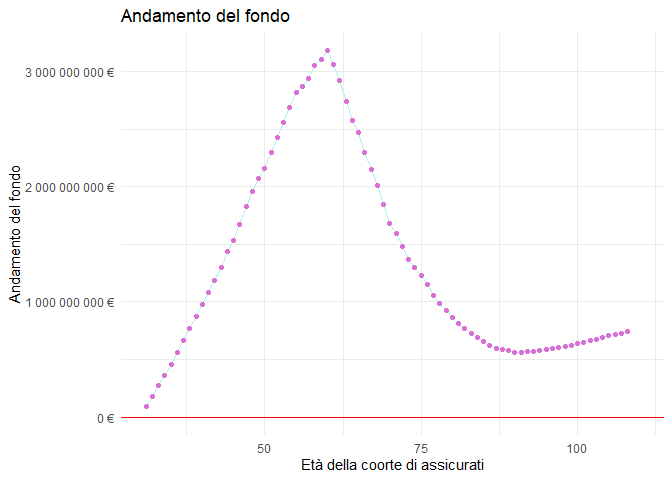
\includegraphics{prova1_files/figure-latex/unnamed-chunk-3-1.pdf}

\begin{Shaded}
\begin{Highlighting}[]
\FunctionTok{plot}\NormalTok{(}\AttributeTok{y =}\NormalTok{ o}\SpecialCharTok{$}\NormalTok{rendimentoFondo,}\AttributeTok{x =} \FunctionTok{c}\NormalTok{(}\DecValTok{31}\SpecialCharTok{:}\DecValTok{70}\NormalTok{),}\AttributeTok{type=}\StringTok{"l"}\NormalTok{)}
\FunctionTok{abline}\NormalTok{(}\AttributeTok{h=}\DecValTok{0}\NormalTok{)}
\end{Highlighting}
\end{Shaded}

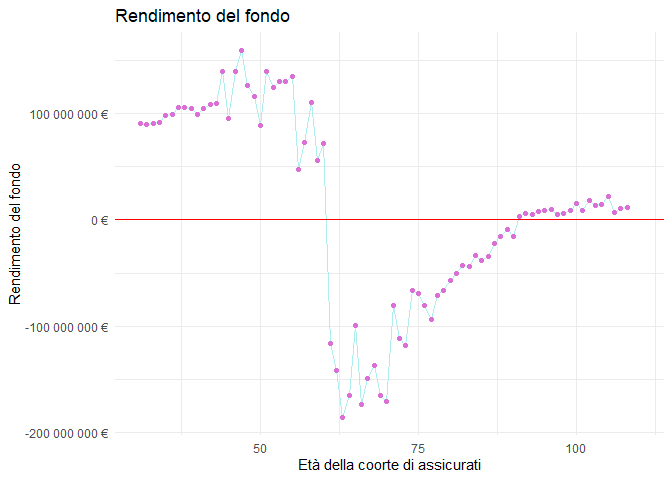
\includegraphics{prova1_files/figure-latex/unnamed-chunk-3-2.pdf}

\hypertarget{metodo-monte-carlo}{%
\subsubsection{Metodo Monte Carlo}\label{metodo-monte-carlo}}

\begin{Shaded}
\begin{Highlighting}[]
\CommentTok{\#\textquotesingle{} MonteCarlo}
\CommentTok{\#\textquotesingle{}}
\CommentTok{\#\textquotesingle{} @param x }
\CommentTok{\#\textquotesingle{} @param level }
\CommentTok{\#\textquotesingle{} @param numeroMomenti }
\CommentTok{\#\textquotesingle{}}
\CommentTok{\#\textquotesingle{} @return }
\CommentTok{\#\textquotesingle{} @export}
\CommentTok{\#\textquotesingle{}}
\CommentTok{\#\textquotesingle{} @examples}
\NormalTok{MonteCarlo }\OtherTok{\textless{}{-}} \ControlFlowTok{function}\NormalTok{(x,}
                       \AttributeTok{level =} \FloatTok{0.95}\NormalTok{,}
                       \AttributeTok{numeroMomenti =} \DecValTok{10}\NormalTok{)}
\NormalTok{\{}
\NormalTok{  monteCarlo }\OtherTok{=} \FunctionTok{new.env}\NormalTok{()}
\NormalTok{  nSimulazioni }\OtherTok{=} \FunctionTok{length}\NormalTok{(x)}
\NormalTok{  monteCarlo}\SpecialCharTok{$}\NormalTok{valAtteso }\OtherTok{=} \FunctionTok{mean}\NormalTok{(x)}
\NormalTok{  monteCarlo}\SpecialCharTok{$}\NormalTok{varianzaCampionaria }\OtherTok{=} \FunctionTok{sd}\NormalTok{(x) }\SpecialCharTok{/} \FunctionTok{sqrt}\NormalTok{(nSimulazioni }\SpecialCharTok{{-}} \DecValTok{1}\NormalTok{)}
  \CommentTok{\#lower tail = false indica che la prob diverta 1{-}alpha al posto di alpha}
\NormalTok{  z }\OtherTok{=} \FunctionTok{qnorm}\NormalTok{((}\DecValTok{1} \SpecialCharTok{{-}}\NormalTok{ level) }\SpecialCharTok{/} \DecValTok{2}\NormalTok{, }\AttributeTok{lower.tail =} \ConstantTok{FALSE}\NormalTok{)}
\NormalTok{  intConfLow }\OtherTok{=}\NormalTok{ monteCarlo}\SpecialCharTok{$}\NormalTok{valAtteso }\SpecialCharTok{{-}}\NormalTok{ z }\SpecialCharTok{*}\NormalTok{ monteCarlo}\SpecialCharTok{$}\NormalTok{varianzaCampionaria}
\NormalTok{  intConfUp }\OtherTok{=}\NormalTok{ monteCarlo}\SpecialCharTok{$}\NormalTok{valAtteso }\SpecialCharTok{+}\NormalTok{ z }\SpecialCharTok{*}\NormalTok{ monteCarlo}\SpecialCharTok{$}\NormalTok{varianzaCampionaria}
\NormalTok{  monteCarlo}\SpecialCharTok{$}\NormalTok{intervalloConfidenza }\OtherTok{=} \FunctionTok{c}\NormalTok{(intConfLow, intConfUp)}
  \ControlFlowTok{for}\NormalTok{ (i }\ControlFlowTok{in} \DecValTok{1}\SpecialCharTok{:}\NormalTok{numeroMomenti)}
\NormalTok{  \{}
\NormalTok{    monteCarlo}\SpecialCharTok{$}\NormalTok{momenti[i] }\OtherTok{=} \FunctionTok{mean}\NormalTok{(x }\SpecialCharTok{**}\NormalTok{ i)}
\NormalTok{  \}}
  
  \CommentTok{\#probabilità di rovina}
\NormalTok{  rovine}\OtherTok{=}\DecValTok{0}
  \ControlFlowTok{for}\NormalTok{ (i }\ControlFlowTok{in} \DecValTok{1}\SpecialCharTok{:}\FunctionTok{length}\NormalTok{(x))}
\NormalTok{  \{}
\NormalTok{    rovine }\OtherTok{=}\NormalTok{ rovine}\SpecialCharTok{+}\FunctionTok{ifelse}\NormalTok{(x[i] }\SpecialCharTok{\textless{}} \DecValTok{0}\NormalTok{, }\DecValTok{1}\NormalTok{, }\DecValTok{0}\NormalTok{)}
\NormalTok{  \}}
\NormalTok{  monteCarlo}\SpecialCharTok{$}\NormalTok{rovina }\OtherTok{=}\NormalTok{ rovine }\SpecialCharTok{/} \FunctionTok{length}\NormalTok{(x)}
  \FunctionTok{return}\NormalTok{(monteCarlo)}
\NormalTok{\}}
\end{Highlighting}
\end{Shaded}

Per la simulazione si è definita una funzione \texttt{monteCarlo} con lo
scopo, a partire da una simulazione arbitrariamente grande (\(10^5\) per
motivi di computazione) della variabile osservata, di stabilire, grazie
alla legge dei grandi numeri, il vero valore teorico della distribuzione
simulata.

\begin{Shaded}
\begin{Highlighting}[]
\NormalTok{x}\OtherTok{=}\DecValTok{0}
\ControlFlowTok{for}\NormalTok{ (i }\ControlFlowTok{in} \DecValTok{1}\SpecialCharTok{:}\DecValTok{10}\SpecialCharTok{**}\DecValTok{3}\NormalTok{)}
\NormalTok{\{}
\NormalTok{  x[i] }\OtherTok{=} \FunctionTok{gestionePortafoglio}\NormalTok{(}
    \AttributeTok{fondoInizio =} \DecValTok{1000}\NormalTok{,}
    \AttributeTok{numeroAssicurati =} \DecValTok{100}\NormalTok{,}
    \AttributeTok{tassoAleatorio =} \FloatTok{0.01}\NormalTok{,}
    \AttributeTok{tassoTecnico =} \FloatTok{0.02}
\NormalTok{  )}\SpecialCharTok{$}\NormalTok{andamentoFondo[}\DecValTok{90}\NormalTok{]}
\NormalTok{\}}
\FunctionTok{MonteCarlo}\NormalTok{(x)}\SpecialCharTok{$}\NormalTok{valAtteso}
\end{Highlighting}
\end{Shaded}

\begin{verbatim}
## [1] 840749.3
\end{verbatim}

\begin{Shaded}
\begin{Highlighting}[]
\FunctionTok{MonteCarlo}\NormalTok{(x)}\SpecialCharTok{$}\NormalTok{intervalloConfidenza}
\end{Highlighting}
\end{Shaded}

\begin{verbatim}
## [1] 811162.1 870336.5
\end{verbatim}

\begin{Shaded}
\begin{Highlighting}[]
\FunctionTok{MonteCarlo}\NormalTok{(x)}\SpecialCharTok{$}\NormalTok{rovina}
\end{Highlighting}
\end{Shaded}

\begin{verbatim}
## [1] 0.03
\end{verbatim}

\hypertarget{funzione-aggiuntiva-capitale-minimo}{%
\subsubsection{Funzione aggiuntiva: Capitale
minimo}\label{funzione-aggiuntiva-capitale-minimo}}

Per sfruttare al meglio \texttt{MonteCarlo} e
\texttt{gestionePortafoglio} è stata sviluppata la funzione
\texttt{CapitaleMinimo}, il suo obiettivo è quello di definire il
capitale iniziale da allocare al portafoglio in modo tale che la
probabilità di rovina (all'ultimo anno della rendita) sia al di sotto di
quella prefissata (in questa caso consideriamo il 5\%). Il problema lo
si potrebbe estendere anche agli anni precedenti all'ultimo della
rendita, in modo che la probabilità di rovina sia sempre sotto la
soglia; per fare ciò basterebbe inserire la funzione CapitaleMinimo
all'interno di un ciclo \texttt{for} con l'indice che va da 1 agli anni
della rendita. Inoltre, l'idea della funzione è che dati i parametri a
meno di uno, la funzione calcola il \emph{p-value} per la variabile
incognita. Quindi, la funzione con piccole modifiche può essere estesa
anche agli altri parametri della funzione \texttt{gestionePortafoglio}.
Per cercare il capitale minimo si utilizza un processo ricorsivo in cui
iniziando da \(0\) (il capitale minimo), lo si aumenta e si verifica se
rispetta la condizione della probabilità di rovina, il capitale viene
aumentato secondo una formula in modo tale da snellire e abbreviare la
procedura, ottenendo così un risultato meno preciso.

\begin{Shaded}
\begin{Highlighting}[]
\CommentTok{\#\textquotesingle{} Capitale Minimo}
\CommentTok{\#\textquotesingle{}}
\CommentTok{\#\textquotesingle{} @param numeroAssicurati }
\CommentTok{\#\textquotesingle{} @param eta }
\CommentTok{\#\textquotesingle{} @param rata }
\CommentTok{\#\textquotesingle{} @param numeroPremi }
\CommentTok{\#\textquotesingle{} @param omega }
\CommentTok{\#\textquotesingle{} @param differimento }
\CommentTok{\#\textquotesingle{} @param temporanea }
\CommentTok{\#\textquotesingle{} @param anniCopertura }
\CommentTok{\#\textquotesingle{} @param rateGarantiteDurata }
\CommentTok{\#\textquotesingle{} @param rendimentoFondoAnnuo }
\CommentTok{\#\textquotesingle{} @param tassoAleatorio }
\CommentTok{\#\textquotesingle{} @param tavolaMortalita }
\CommentTok{\#\textquotesingle{} @param tassoTecnico }
\CommentTok{\#\textquotesingle{} @param tavolaPeriodo }
\CommentTok{\#\textquotesingle{} @param andamentoFondo }
\CommentTok{\#\textquotesingle{} @param rendimentoFondo }
\CommentTok{\#\textquotesingle{} @param decessi }
\CommentTok{\#\textquotesingle{} @param precisione }
\CommentTok{\#\textquotesingle{}}
\CommentTok{\#\textquotesingle{} @return}
\CommentTok{\#\textquotesingle{} @export}
\CommentTok{\#\textquotesingle{}}
\CommentTok{\#\textquotesingle{} @examples}
\NormalTok{capitaleMinimo }\OtherTok{=} \ControlFlowTok{function}\NormalTok{ (}\AttributeTok{numeroAssicurati =} \DecValTok{1000}\NormalTok{,}
                           \AttributeTok{eta =} \DecValTok{20}\NormalTok{,}
                           \AttributeTok{rata =} \DecValTok{1000}\NormalTok{,}
                           \AttributeTok{numeroPremi =} \DecValTok{15}\NormalTok{,}
                           \AttributeTok{omega =} \DecValTok{110}\NormalTok{,}
                           \AttributeTok{differimento =} \DecValTok{25}\NormalTok{,}
                           \AttributeTok{temporanea =} \ConstantTok{FALSE}\NormalTok{,}
                           \CommentTok{\# temporanea o  vita intera}
                           \AttributeTok{anniCopertura =} \DecValTok{35}\NormalTok{,}
                           \AttributeTok{rateGarantiteDurata =} \DecValTok{5}\NormalTok{,}
                           \AttributeTok{rendimentoFondoAnnuo =} \FloatTok{0.01}\NormalTok{,}
                           \CommentTok{\# tasso finanziario}
                           \AttributeTok{tassoAleatorio =} \ConstantTok{TRUE}\NormalTok{,}
                           \AttributeTok{tavolaMortalita =}\NormalTok{ demoIta}\SpecialCharTok{$}\NormalTok{RG48M,}
                           \CommentTok{\#tavola utilizzata per la base tecnica}
                           \AttributeTok{tassoTecnico =} \FloatTok{0.02}\NormalTok{,}
                           \CommentTok{\#tasso utilizzato per la base tecnica}
                           \AttributeTok{tavolaPeriodo =}\NormalTok{ demoIta}\SpecialCharTok{$}\NormalTok{SIM02,}
                           \AttributeTok{precisione =} \DecValTok{1000}\NormalTok{, }\AttributeTok{anno =} \DecValTok{90}\NormalTok{)}
\NormalTok{\{}
\NormalTok{  capitaleMinimo }\OtherTok{=} \DecValTok{0}
\NormalTok{  x }\OtherTok{=} \DecValTok{0}
  \ControlFlowTok{for}\NormalTok{ (i }\ControlFlowTok{in} \DecValTok{1}\SpecialCharTok{:}\NormalTok{precisione)}
\NormalTok{  \{}
\NormalTok{    x[i] }\OtherTok{=}
      \FunctionTok{gestionePortafoglio}\NormalTok{(}
        \AttributeTok{numeroAssicurati =}\NormalTok{ numeroAssicurati,}
        \AttributeTok{eta =}\NormalTok{ eta,}
        \AttributeTok{rata =}\NormalTok{ rata,}
        \AttributeTok{numeroPremi =}\NormalTok{ numeroPremi,}
        \AttributeTok{omega =}\NormalTok{ omega,}
        \AttributeTok{differimento =}\NormalTok{ differimento,}
        \AttributeTok{temporanea =}\NormalTok{ temporanea,}
        \AttributeTok{anniCopertura =}\NormalTok{ anniCopertura,}
        \AttributeTok{rateGarantiteDurata =}\NormalTok{ rateGarantiteDurata,}
        \AttributeTok{rendimentoFondoAnnuo =}\NormalTok{ rendimentoFondoAnnuo,}
        \AttributeTok{tassoAleatorio =}\NormalTok{ tassoAleatorio,}
        \AttributeTok{tavolaMortalita =}\NormalTok{ tavolaMortalita,}
        \AttributeTok{tassoTecnico =}\NormalTok{ tassoTecnico,}
        \AttributeTok{tavolaPeriodo =}\NormalTok{ tavolaPeriodo,}
        \AttributeTok{fondoInizio =}\NormalTok{ capitaleMinimo}
\NormalTok{      )}\SpecialCharTok{$}\NormalTok{andamentoFondo[anno]}
\NormalTok{  \}}
  \ControlFlowTok{while}\NormalTok{ (}\FunctionTok{MonteCarlo}\NormalTok{(x)}\SpecialCharTok{$}\NormalTok{rovina }\SpecialCharTok{\textgreater{}} \FloatTok{0.05}\NormalTok{)}
\NormalTok{  \{}
\NormalTok{    capitaleMinimo }\OtherTok{=}\NormalTok{ capitaleMinimo }\SpecialCharTok{+} \FunctionTok{abs}\NormalTok{(}\FunctionTok{quantile}\NormalTok{(x, }\AttributeTok{probs =} \FloatTok{0.05}\NormalTok{)) }\SpecialCharTok{/} \FunctionTok{ifelse}\NormalTok{(}\FunctionTok{MonteCarlo}\NormalTok{(x)}\SpecialCharTok{$}\NormalTok{rovina }\SpecialCharTok{\textgreater{}} \FloatTok{0.9}\NormalTok{,}
                                                      \DecValTok{8}\NormalTok{,}
                                                      \FunctionTok{ifelse}\NormalTok{(}
                                                        \FunctionTok{MonteCarlo}\NormalTok{(x)}\SpecialCharTok{$}\NormalTok{rovina }\SpecialCharTok{\textgreater{}} \FloatTok{0.1}\NormalTok{,}
                                                        \DecValTok{20}\NormalTok{,}
                                                        \FunctionTok{ifelse}\NormalTok{(}\FunctionTok{MonteCarlo}\NormalTok{(x)}\SpecialCharTok{$}\NormalTok{rovina }\SpecialCharTok{\textgreater{}} \FloatTok{0.08}\NormalTok{, }\DecValTok{30}\NormalTok{, }\DecValTok{40}\NormalTok{)}
\NormalTok{                                                      ))}
    \FunctionTok{print}\NormalTok{(capitaleMinimo)}
\NormalTok{    probabilitaRovina }\OtherTok{=} \FunctionTok{MonteCarlo}\NormalTok{(x)}\SpecialCharTok{$}\NormalTok{rovina}
    \FunctionTok{print}\NormalTok{(probabilitaRovina)}
    \ControlFlowTok{for}\NormalTok{ (i }\ControlFlowTok{in} \DecValTok{1}\SpecialCharTok{:}\NormalTok{precisione)}
\NormalTok{    \{}
\NormalTok{      x[i] }\OtherTok{=} \FunctionTok{gestionePortafoglio}\NormalTok{(}
        \AttributeTok{numeroAssicurati =}\NormalTok{ numeroAssicurati,}
        \AttributeTok{eta =}\NormalTok{ eta,}
        \AttributeTok{rata =}\NormalTok{ rata,}
        \AttributeTok{numeroPremi =}\NormalTok{ numeroPremi,}
        \AttributeTok{omega =}\NormalTok{ omega,}
        \AttributeTok{differimento =}\NormalTok{ differimento,}
        \AttributeTok{temporanea =}\NormalTok{ temporanea,}
        \AttributeTok{anniCopertura =}\NormalTok{ anniCopertura,}
        \AttributeTok{rateGarantiteDurata =}\NormalTok{ rateGarantiteDurata,}
        \AttributeTok{rendimentoFondoAnnuo =}\NormalTok{ rendimentoFondoAnnuo,}
        \AttributeTok{tassoAleatorio =}\NormalTok{ tassoAleatorio,}
        \AttributeTok{tavolaMortalita =}\NormalTok{ tavolaMortalita,}
        \AttributeTok{tassoTecnico =}\NormalTok{ tassoTecnico,}
        \AttributeTok{tavolaPeriodo =}\NormalTok{ tavolaPeriodo,}
        \AttributeTok{fondoInizio =}\NormalTok{ capitaleMinimo}
\NormalTok{      )}\SpecialCharTok{$}\NormalTok{andamentoFondo[anno]}
\NormalTok{    \}}
\NormalTok{  \}}
  \FunctionTok{return}\NormalTok{(capitaleMinimo)}
\NormalTok{\}}

\FunctionTok{capitaleMinimo}\NormalTok{(}\AttributeTok{rendimentoFondoAnnuo =} \FloatTok{0.015}\NormalTok{,}\AttributeTok{tassoTecnico =} \FloatTok{0.02}\NormalTok{,}\AttributeTok{precisione =} \DecValTok{100}\NormalTok{)}
\end{Highlighting}
\end{Shaded}

\begin{verbatim}
##     5% 
## 411272 
## [1] 0.81
##       5% 
## 696100.8 
## [1] 0.66
##       5% 
## 932533.3 
## [1] 0.48
##      5% 
## 1143927 
## [1] 0.43
##      5% 
## 1240716 
## [1] 0.3
##      5% 
## 1374564 
## [1] 0.2
##      5% 
## 1495257 
## [1] 0.24
##      5% 
## 1624811 
## [1] 0.18
##      5% 
## 1737185 
## [1] 0.17
##      5% 
## 1850619 
## [1] 0.12
##      5% 
## 1948427 
## [1] 0.18
##      5% 
## 2024959 
## [1] 0.13
\end{verbatim}

\begin{verbatim}
##      5% 
## 2024959
\end{verbatim}

\end{document}
